\newpage
\section{INTRODUÇÃO}


A internet é uma rede mundial que interliga milhões de computadores em todo o mundo, servindo como um grande fator de comunicação e integração social \cite{marioFalcao2015}. Todos os dias, novas páginas na internet surgem, sejam de relacionamento, humor, entretenimento, notícias, ou redes sociais, como exemplo: Facebook, Twitter, Instagram, Google+, Vimeo, DailyMotion e Youtube.

É pertinente que em nossa sociedade contemporânea, as pessoas estejam mais próximas da tecnologia, principalmente as crianças. 
Essas crianças adquirem habilidades diferentes das crianças de antigamente: enquanto uma criança da década de 80 possuía uma maior facilidade para construir ou modelar um brinquedo, as crianças da geração atual possuem habilidades para lidar com a informática, devido ao convívio rotineiro com a mesma \cite{marioFalcao2016}.

% Motivação para utilização do Youtube
A plataforma de vídeos Youtube é o segundo site mais acessado do mundo \cite{alexaYoutube}. Em tal plataforma, é possível postar e compartilhar vídeos com uma enorme e abrangente gama de conteúdos, servindo também como site de buscas. É possível encontrar conteúdo musical, \textit{vlogs}, animações, curta-metragens, conteúdo educativo, conteúdo com público alvo adulto e conteúdo voltado especificamente ao público jovem e infantil, como por exemplo os canais \textbf{Felipe Neto} \footnote{https://www.youtube.com/channel/UCV306eHqgo0LvBf3Mh36AHg} e \textbf{Galinha Pintadinha} \footnote{https://www.youtube.com/channel/UCBAb\_DK4GYZqZR9MFA7y2Xg}.

Como parte de suas características de rede social, o Youtube disponibiliza, em seus vídeos, a possibilidade de usuários comentarem. Porém, tendo em vista as crianças e adolescentes estão conectadas na rede cada vez mais cedo \cite{EnyoGoncalves2017}, ao navegar pela plataforma em vídeos infantis, nota-se que há uma certa liberdade para realizar comentários de qualquer natureza, até mesmo ofensivos ou inapropriados para o público o qual o vídeo é destinado, um exemplo disso pode ser visto na Figura \ref{fig:youtube_comment}.

Segundo o artigo 17 do \textbf{Estatuto da Criança e do Adolescente} (ECA): "O direito ao respeito consiste na inviolabilidade da integridade física, psíquica e moral da criança e do adolescente, abrangendo a preservação da imagem, da identidade, da autonomia, dos valores, ideias e crenças, dos espaços e objetos pessoais." \cite{eca_lei}.  Assim, é possível através da tecnologia buscar meios para proteger moralmente e psiquicamente o público mais jovem que utiliza a plataforma. 

\begin{figure}[H] %use h para forçar que a figura fique abaixo do texto
	\caption{\label{fig:youtube_comment} Comentário em um vídeo infantil no Youtube}
	\begin{center}
	    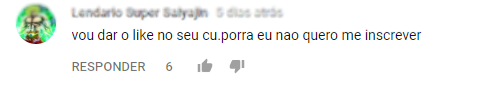
\includegraphics[scale=1]{figuras/figura_1.png} % altere o atributo scale para o tamanho da figura
	\end{center}
	\legend{Fonte: Youtube - 13 de Setembro de 2017}
%Verificar se precisa por a data aqui 
\end{figure}

A Figura \ref{fig:youtube_comment} foi retirada do vídeo \textbf{UPA CAVALINHO - Clipe Música Oficial - Galinha Pintadinha DVD 4}, um vídeo direcionado à crianças de 2 a 7 anos postado pelo canal \emph{Galinha Pintadinha}, que é direcionado ao público infantil. Por questões de anonimato o usuário não é identificado. %Explicar o comentário que pode ser visualizado e interpretado pela criança. Também seria bom referências para isso. %N.A. (28nov2017) não encontrei referências para "crianças palavrão"; checar os links abaixo:
%http://onlinelibrary.wiley.com/doi/10.1111/j.1365-2214.2011.01338.x/full
%http://www.tandfonline.com/doi/abs/10.1080/01434630408666529
%procurar tb por children+swear words.
%Talvez colocar uma imagem do vídeo do felipe neto


O objetivo deste trabalho é identificar comentários pejorativos semelhantes ao apresentado na Figura \ref{fig:youtube_comment} em vídeos postados no Youtube, direcionados à crianças e adolescentes. Para alcançar este objetivo, primeiramente foi criado um script na linguagem \textit{Python}, para coleta de comentários dos vídeos através da API do Youtube. Outro script \textit{Python} também foi utilizado para realizar o pré-processamento dos comentários, através da biblioteca de processamento de linguagem natural \textbf{NLTK}. Com o \textit{dataset} de comentários coletados e pré-processados, foi criado um modelo de classificação utilizando as ferramentas \textbf{SentiStrength} e \textbf{scikit-learn}. A \textbf{scikit-learn} também foi utilizada para avaliar a eficiência do modelo criado. A utilização das ferramentas é descrita de forma detalhada no Capítulo 5. 

Utilizando tecnologias web (HTML, CSS, Javascript), foi desenvolvido também uma extensão para o navegador da web \textbf{Google Chrome}. A extensão exibe os resultados da classificação previamente realizada, para o vídeo sendo assistido naquele momento. Os dados da classificação ficam salvos em um banco de dados. 

%Falar das ferramentas que serão utilizadas

%\begin{itemize}
 %   \item Questão de Pesquisa?
  %  \item Questão de Pesquisa? 
   % \item Questão de Pesquisa?
%\end{itemize}

%Neste trabalho o idioma dos textos analisados é estritamente português, e na Seção 5 serão esclarecidos os critérios que são considerados para que um comentário seja classificado como pejorativo.

Este trabalho está estruturado da seguinte forma. No Capítulo 2, são apresentados os objetivos do trabalho; no Capítulo 3, são apresentados os principais conceitos que são utilizados durante o projeto; no Capítulo 4, serão apresentados os principais trabalhos relacionados, que tratam dos temas de mineração e de proteção de crianças online; o Capítulo 5 apresenta a metodologia de trabalho; o Capítulo 6 apresenta os resultados obtidos pelo modelo de classificação textual; O Capítulo 7 apresenta uma conclusão do autor sobre o trabalho e seus resultados; E o Capítulo 8 apresenta sugestões de melhorias assim como linhas de execução para trabalhos futuros.



\begin{comment}
\textcolor{red}{mover objetivos e fundamentacao teorica para depois da introdução} - DONE
\end{comment}
